\chapter{Les outils de mesure de la performance}
\label{part:outils}

Après avoir étudié les facteurs de la performance en athlétisme, nous allons maintenant nous intéresser aux différents outils qui permettent de mesurer les facteurs physiologiques cités précédemment. \\

    \section{Lecteur de glycémie}
    
    Un lecteur de glycémie est un appareil permettant de mesurer la glycémie (cf. p.\pageref{glycemie}  \ref{glycemie}). Le taux y est affiché à l’écran et est exprimé en millimole de glucose par litre de sang, en milligramme de glucose par décilitre de sang (mg/dl) ou encore en gramme de glucose par litre de sang (g/l). \\
    
    Parfois, l’écran n’affiche pas de chiffres, mais seulement les mots « Low » ou « High », signifiant que le taux de glucose est trop faible ou trop élevé.\\
    
    Il existe deux systèmes de mesure du taux de glucose : 
    \begin{itemize}
        \item classique,
        \item en continu.\\
    \end{itemize}
    
    Les lecteurs de glycémie classiques et les systèmes de mesure du glucose en continu servent tout deux à évaluer le taux de glucose. Cependant, ces analyses ne proviennent pas des mêmes fluides corporels (fig. \ref{fig:capillaireVSinterstitiel}).\\
    
    Le glucomètre se base sur le glucose sanguin contenu dans les capillaires (figure B), c'est à dire les plus petits vaisseaux du corps humain, alors que les systèmes de mesure du glucose en continu ou systèmes de mesure de la glycémie interstitielle (figure A) se basent sur le glucose contenu dans le liquide interstitiel. Ce dernier est un liquide qui se trouve entre les cellules et les capillaires sanguins et dans lequel le glucose circule librement (fig. \ref{fig:capillaireVSinterstitiel}).
    
     \begin{figure}[H]
        \centering
        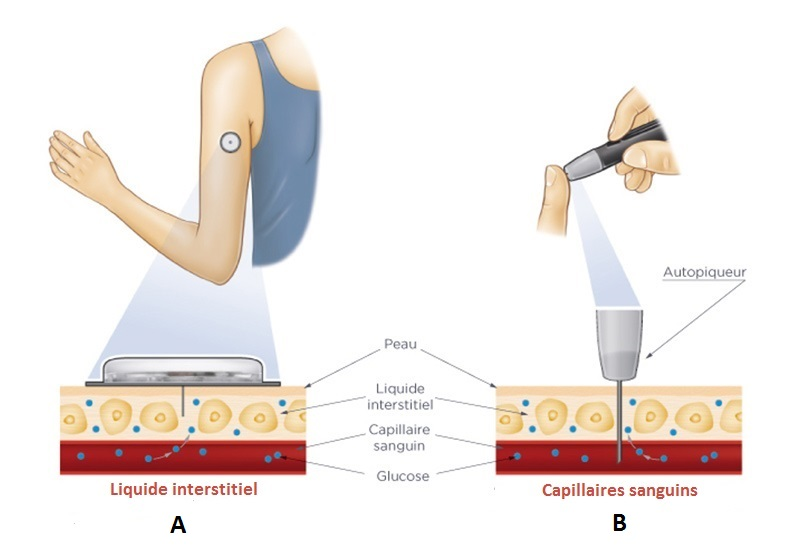
\includegraphics[scale=0.7]{images/glucometreVSfreestyle2.jpg}
        \caption{\label{fig:capillaireVSinterstitiel}Différents types de mesure de la glycémie. Glycémie interstitielle en continue (figure A), glycémie capillaire classique (figure B). }
    \end{figure}
    
    
    La glycémie capillaire est la méthode la plus utilisée et nécessite l'utilisation d'un auto-piqueur (muni d'aiguilles à usage unique appelées lancettes), de bandelettes et d'un lecteur de glycémie. \\
    
    Un petit échantillon de sang est prélevé et déposé sur la bandelette puis analysé par le glucomètre (fig. \ref{fig:glycemieCapillaire}).
    
    \begin{figure}[H]
        \centering
        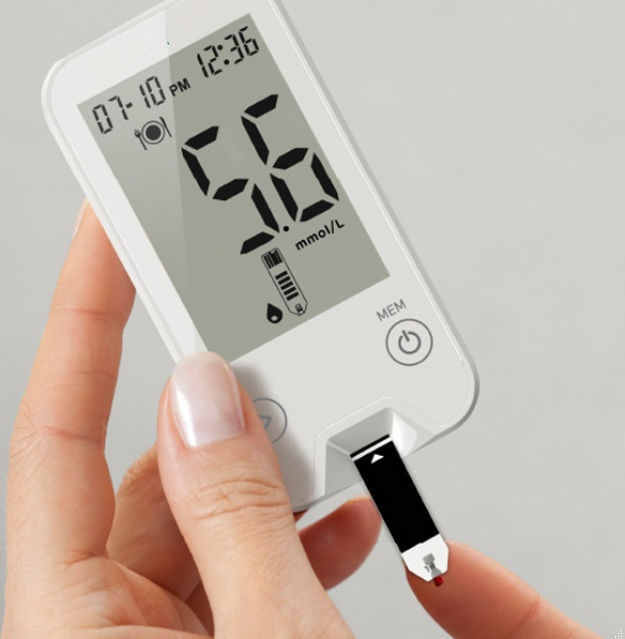
\includegraphics[scale=0.25]{images/glucometre.jpg}
        \caption{\label{fig:glycemieCapillaire}Système de mesure de la glycémie capillaire}
    \end{figure}

    
    Un système de mesure du glucose en continu est composé d’un capteur posé à l'arrière du bras pendant 14 jours et d'un lecteur qui permet de scanner le capteur et de collecter les données (fig. \ref{fig:systemeContinu}).
    
    \begin{figure}[H]
        \centering
        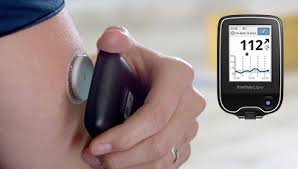
\includegraphics[scale=0.8]{images/glucometre2.jpg}
        \caption{\label{fig:systemeContinu}Système de mesure du glucose en continu}
    \end{figure}
    
    
    Les études ont montré que la quantité de glucose dans le milieu interstitiel reflétait le taux de glucose dans le sang, mais avec un décalage de quelques minutes (au maximum 10 minutes) dans certaines situations:
    \begin{itemize}
        \item lorsque la glycémie est en train de baisser,
        \item lorsque la glycémie est en train d'augmenter.\\
    \end{itemize}
    Ce décalage est principalement lié au temps de transfert du glucose entre le sang et le liquide interstitiel.\\
    
    Après une course, nous nous trouvons justement dans une de ces situations, car la glycémie se modifie. Un système de mesure de la glycémie interstitielle n'est alors pas adapté pour les athlètes qui souhaitent connaître leur glycémie immédiatement après un effort. Par conséquent, nous utiliserons un glucomètre classique pour l'étude de la glycémie dans le \autoref{part:experimentation}.
    
    
    \vspace{10pt}
    
    
    \section{Lactatomètre}
    
    Un lactatomètre est un appareil permettant de mesurer la lactatémie (cf. p.\pageref{lactatemie}  \ref{lactatemie}). Elle est exprimée à l'écran en millimoles par litre de sang (mmol/L).\\
    
    Les lactatomètres nécessitent l'utilisation d'un auto-piqueur pour le prélèvement du sang sur l'index ou le lobe de l'oreille de l'athlète ainsi que de bandelettes réactives, c'est à dire recouvertes d'une substance utilisée pour produire une réaction chimique. \\
    
    Un petit échantillon de sang est prélevé et déposé sur la bandelette puis analysé par le lactatomètre.\\

    Un des outils les plus répandus dans le monde du sport est le « Lactate Pro 2 » (fig. \ref{fig:lactatePro2}), car les résultats obtenus avec celui-ci sont aussi précis que ceux obtenus sur des appareils plus sophistiqués. 
    
     \begin{figure}[H]
        \centering
        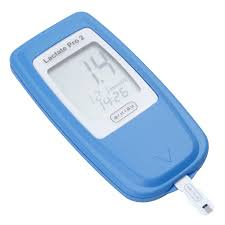
\includegraphics[scale=0.6]{images/lactatePro.jpg}
        \caption{\label{fig:lactatePro2}Lecteur de lactatemie « Lactate Pro 2 »}
    \end{figure}
    
    Le Lactate Pro 2 mesure le taux de lactate en seulement 15 secondes par prélèvement d'une très faible quantité de sang (volume d‘échantillon d'uniquement 0,3 \si{\micro}l). Le sang est automatiquement aspiré par la bandelette, ce qui réduit le risque d'erreur et garantit une mesure fiable sans contamination. \\
        
    De plus, toutes les données peuvent être transmises et archivées vers un PC de façon structurée grâce à l'interface USB intégrée. \\
    
    C'est cet outil que j'utiliserai dans le \autoref{part:experimentation}.\\
    
    
    \section{Oxymètre de pouls}

    L'oxymètre de pouls ou saturomètre est un appareil destiné à mesurer la fréquence cardiaque et l'oxymétrie de pouls (cf. p.\pageref{oxymetrie}  \ref{oxymetrie}). Il se présente généralement sous la forme d'un pince à doigt avec un capteur à l'intérieur et un écran qui affiche la saturation pulsée de l’hémoglobine en oxygène (SpO2) (fig \ref{fig:oxymetre}).
    
    \begin{figure}[H]
        \centering
        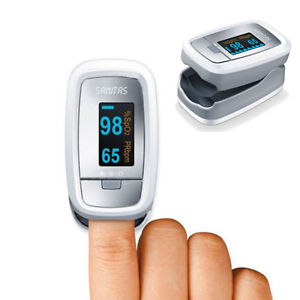
\includegraphics[scale=0.55]{images/oxymetre2.jpg}\hfill
        \caption{\label{fig:oxymetre}Oxymètre de pouls}
    \end{figure}
    
    L'avantage de cet outil est qu'il ne fait appel à aucun prélèvement sanguin.\\
    
    L'oxymètre de poul repose sur le principe d'absorption de la lumière c'est-à-dire sur la quantité de lumière absorbée pour une longueur d'onde donnée.
    L'émetteur de l'oxymètre émet deux faisceaux de lumière (rouge et infrarouge) de longueur d'onde différente (respectivement de 660 et 940 nm) à travers la peau et qui sont réceptionnés par un récepteur (fig \ref{fig:oxymetre_fonctionnement}).
    
     \begin{figure}[H]
        \centering
        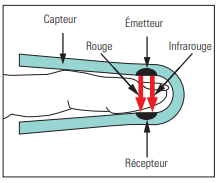
\includegraphics[scale=1]{images/oxymetre3.jpg}
        \caption{\label{fig:oxymetre_fonctionnement}Fonctionnement de l'oxymètre de pouls}
    \end{figure}
    
    L’hémoglobine riche en oxygène (oxyhémoglobine), absorbe la lumière infrarouge et laisse passer la lumière rouge alors que l’hémoglobine faible en oxygène (désoxyhémoglobine) absorbe la lumière rouge et est perméable à la lumière infrarouge. En calculant la différence d’absorption de ces deux lumières, l’oxymètre de pouls peut mesurer le niveau d’oxygénation du sang.

       
    \vspace{10pt}
     
    \section{Cardio-fréquencemètre}
    
        Le cardio-fréquencemètre est un outil incontournable du sportif, car il permet de mesurer instantanément sa fréquence cardiaque (cf. p.\pageref{frequence_cardiaque}  \ref{frequence_cardiaque}). \\
        
        Il existe des cardio-fréquencemètres avec ceinture thoracique et d'autres sans. 
        
        \subsection{Cardio-fréquencemètre avec ceinture thoracique}
        
            Le cardio-fréquencemètre avec ceinture (fig. \ref{fig:cardio_ceinture}) est généralement le plus utilisé et mesure l’activité électrique du coeur grâce à des électrodes qui permettent de capter les impulsions cardiaques. Les électrodes sont placées sur une ceinture émettrice positionnée sous la poitrine et qui est chargée de transmettre les données à un récepteur. Celui-ci est généralement porté au poignet sous forme de montre qui sert d'écran de contrôle et affiche la fréquence cardiaque.
            
            \begin{figure}[H]
                \centering
                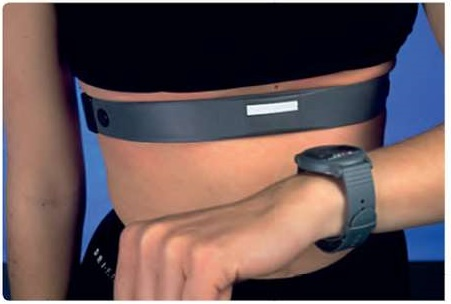
\includegraphics[scale=0.5]{images/cardio-ceinture2.jpg}
                \caption{\label{fig:cardio_ceinture}Cardio-fréquencemètre avec ceinture thoracique}
            \end{figure}
        
        Les cardio-fréquencemètres avec ceinture thoracique sont très performants et entièrement satisfaisants, mais le port d'une ceinture peut être contraignant pour un athlète. En effet, la ceinture peut gêner la respiration et certains athlètes peuvent développer des allergies au contact de celle-ci. Il arrive également que la fréquence cardiaque ne soit pas détectée en raison d'une trop faible humidification des électrodes ou d'un mauvais placement. De plus, des ondes circulent pour pouvoir transmettre les données entre la ceinture et le récepteur, ce qui n'est pas idéal d'un point de vue santé. Le signal peut également être parasité par d'autres ondes environnantes (lignes électriques, etc.). \\
        
        Il existe donc des cardio-fréquencemètres fonctionnant sans ceinture thoracique, qui sont moins encombrants et sans effet d'ondes puisqu'ils reposent sur une technologie complètement différente : la lecture optique.

         
        \subsection{Cardio-fréquencemètre sans ceinture thoracique}
         
        La lecture optique est la dernière technologie en matière de mesure de la fréquence cardiaque.
        Son principe de base est d'utiliser la lumière pour mesurer les variations de l'afflux sanguin engendrées par les battements du coeur. En effet, au moment du battement du coeur, la quantité de sang présente dans la zone testée est légèrement modifiée et le niveau de lumière change.\\
        
        Le capteur optique repose donc sur une source de lumière et un capteur de lumière. La source de lumière, composée d'une ou plusieurs LED, émet de la lumière qui va pénétrer les couches de la peau. Une partie de la lumière va être réfléchie et le capteur va réceptionner le signal lumineux. En analysant la quantité de lumière reflétée, le capteur sera capable de déterminer l’afflux sanguin et par conséquent, la fréquence cardiaque.\\
        
        Parmi les outils utilisables par le sportif, il existe la cardiobague qui se porte autour d'un doigt ou encore la montre avec cardio-fréquencemètre au poignet (fig. \ref{fig:cardiobague}).
        
         \begin{figure}[H]
                \centering
                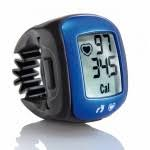
\includegraphics[scale=0.8]{images/cardiobague.jpg}
                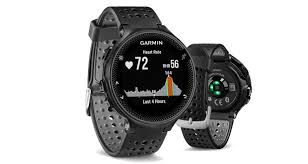
\includegraphics[scale=0.7]{images/garmin.jpg}
                \caption{\label{fig:cardiobague}Cardio-bague et montre cardio}
            \end{figure}


     En comparaison, il y a en moyenne 2 bpm d'écart entre les résultats obtenus par la mesure de la variation due au flux sanguin au bout du bras et ceux provenant de la mesure par impulsion électrique directement à la sortie du coeur. Étant donné que ces résultats sont très similaires, nous préférerons utiliser une montre cardio-fréquencemètre pour l'étude (\autoref{part:experimentation}).
        

   






    
        
%%% Local Variables: 
%%% mode: latex
%%% TeX-master: "rapport"
%%% End: 

